%---------------------------------------------------------------------------------
%                西南交通大学研究生学位论文:第三章内容
%---------------------------------------------------------------------------------
\chapter{TCP/NC协议实现}
本章主要讲TCP/NC的具体实现,在无线lossy信道下测试TCP/NC的性能,并与标准的TCP-vegas进行分析对比。
\section{数据包编码}
在阐述数据包编码之前,先简单介绍近世代数的相关概念。
\subsection{有限域与扩域}
\begin{myDef}[阿贝尔群]
	对于一个非空元素集合$G$以及定义在$G$上的一种运算“$*$”( 这里的$*$泛指一种代数运算,如$+$,$-$,$\times$,$\div$,模$m$加$\oplus$,模$m$乘$\odot$等)。若满足以下四个条件:
	\begin{enumerate}[fullwidth,itemindent=2em,label=(\arabic*)]
		\item 封闭性,即$\forall a,b \in G$,$\exists\left(a*b\right)=c\in G$。
		\item 结合性,即$\forall a,b \in G$,$\exists a*\left(b*c\right)=\left(a*b\right)*c$。
		\item 存在唯一一个单位元$e$,即$\forall a \in G$,$\exists a*e=e*a=a$。
		\item $G$中的每个元素各自存在唯一的逆元,即$\forall a \in G$,$\exists {a^{ - 1}} \in G$,使得$a*{a^{-1}}={a^{-1}}*a=e$。这里${a^{-1}}$泛指逆元。
		\item $\forall a,b \in G$,$\exists a*b=b*a$
	\end{enumerate}
	\par
	则称这样的代数系统为阿贝尔群,记做$\left(G,*\right)$\textsuperscript{\cite{zzc2003}}。
\end{myDef}
\begin{myDef}[有限域]
	非空集合$F$含有有限个元素,其中定义了加和乘两种运算,且满足
	\begin{enumerate}[fullwidth,itemindent=2em,label=(\arabic*)]
		\item $F$关于加法构成阿贝尔群,加法恒等元记为0
		\item $F$中所有非零元素对乘法构成阿贝尔群,乘法恒等元记为1
		\item $F$加法和乘法满足分配律
	\end{enumerate}
	\par
	则$F$与这两种运算构成有限域\textsuperscript{\cite{zzc2003}}。
\end{myDef}
\begin{table}[htbp]
	\centering
	\caption{本原多项式$P\left(x\right)=x^{4}+x+1$的根生成的循环群}
	\begin{tabularx}{250pt}{c|c|c}
		\toprule
		\textbf{各次幂$\alpha_{k}$} & \textbf{$\alpha$的多项式}&\textbf{多项式系数$m$重}\\
		\midrule
		$\alpha^{0}$ & 1 &$\left(0001\right)$\\
		\hline
		$\alpha^{1}$ & $\alpha$ &$\left(0010\right)$\\
		\hline
		$\alpha^{2}$ & $\alpha^{2}$ & $\left(0100\right)$\\
		\hline
		$\alpha^{3}$ & $\alpha^{3}$ & $\left(1000\right)$\\
		\hline
		$\alpha^{4}$ & $\alpha+1$ & $\left(0011\right)$\\
		\hline
		$\alpha^{5}$ & $\alpha^{2}+\alpha$ & $\left(0110\right)$\\
		\hline
		$\alpha^{6}$ & $\alpha^{3}+\alpha^{2}$ & $\left(1100\right)$\\
		\hline
		$\alpha^{7}$ & $\alpha^{3}+\alpha+1$ & $\left(1011\right)$\\
		\hline
		$\alpha^{8}$ & $\alpha^{2}+1$ & $\left(0101\right)$\\
		\hline
		$\alpha^{9}$ & $\alpha^{3}+\alpha$ & $\left(1010\right)$\\
		\hline
		$\alpha^{10}$ & $\alpha^{2}+\alpha+1$ & $\left(0111\right)$\\
		\hline
		$\alpha^{11}$ & $\alpha^{3}+\alpha^{2}+\alpha$ & $\left(1110\right)$\\
		\hline
		$\alpha^{12}$ & $\alpha^{3}+\alpha^{2}+\alpha+1$ & $\left(1111\right)$\\
		\hline
		$\alpha^{13}$ & $\alpha^{3}+\alpha^{2}+1$ & $\left(1101\right)$\\
		\hline
		$\alpha^{14}$ & $\alpha^{3}+1$ & $\left(1001\right)$\\
		\hline
	\end{tabularx}
	\label{SHUYU}
\end{table}
\par
有限域提供了一个有限集,在该有限集上明确地定义且有效地实现了加法、减法、乘法及除法运算( 减法可以转换为加法,除法可以转换为乘法),并允许系统使用矩阵、行列式、高斯消元等线性代数中常见的运算工具来解决该域上的联立线性方程组问题。
\par
我们在讲到$GF\left(q\right)$时,经常顺带会讲到$GF\left(q^{m}\right)$,表示$GF\left(q\right)$的扩域。扩域里至少存在一个本原元$\alpha$,它的各次幂$\alpha^{0}$,$\alpha^{1}$,$\alpha^{2}$,$\dots$,$\alpha^{q^{m}-2}$构成了扩域$GF\left(q^{m}\right)$的全部非零域元素。表\ref{SHUYU}展示的就是以本原多项式$P\left(x\right)=x^{4}+x+1$对应的本原元的各次幂生成的$GF\left(2^4\right)$的全部非零元素。
\subsection{数据包的运算}
由于从TCP层下来的数据包都是字节流,如何抽象出我们在第\ref{xianxingbianma}小节中谈到的报文概念呢?进一步地,我们如何对这些报文进行各种操作,如加减乘除呢?
\par
将数据包分解成字节,先对字节进行加减乘除的操作,拼接得到的结果是可行的。这解决了以何种角度刻画数据包的问题。对于数据包的运算,如果是在实数域上进行各种代数运算,则会涉及到进位的问题,不好处理。例如,$p_{1}$和$p_{2}$这两个数据包的二进制形式为$p_{1}=\left(1010\ 1010\right)$和$p_{2}=\left(1111\ 0000\right)$。在实数域上计算得到$p_{3}=p_{1}+p_{2}$,则$p_{3}=\left(1\ 1001\ 1010\right)$,$p_{1}$和$p_{2}$都是8个比特,但是$p_{3}$却是$9$比特,出现了进位,导致我们的处理很麻烦。
\par
上一小节中提到的有限域和扩域是解决数据包运算问题的关键。有限域是一种代数结构,也存在着和实数域中一样的加减乘除等运算,并且各个元素进行加减乘除得到的结果也在有限域中。具体实现过程如下:
\begin{enumerate}[fullwidth,itemindent=2em,label=(\arabic*)]
	\item 确定有限域的大小。由于在计算机中按字节操作最方便,一个字节8个比特,刚好可以看做是一个8位向量。因此,选定扩域$GF\left(2^8\right)$。
	\item 选定一个在$GF\left(2^8\right)$下的生成元$\alpha$,$\alpha$的各次幂和零元素一起构成整个扩域,即$GF\left(2^8\right)=\{0,1,\alpha,\alpha^2,\alpha^3,\dots,\alpha^{254}\}$。$GF\left(2^8\right)$可用的生成元如表格\ref{GENERATOR}。这里我们选定$\alpha=0x03$作为生成元。换句话说,$\forall e \in GF\left(2^8\right) $,且$e \neq 0$,$e=\left(0x03\right)^{k}\left(k=0,1,2,\dots,254\right)$。
	\item 构建以$0x03$作为生成元的$Exponential$表,$Exp\_tab[256]$和$Logarithm$表,$Log\_tab[256]$。其中$Exp\_tab[i]=\left(0x03\right)^{i}$,$\left(0x03\right)^{Log\_tab[i]}=i$。所有代数运算都在$GF\left(2^8\right)$下进行。$Exp\_tab[256]$和$Log\_tab[256]$如表\ref{Exptab}和表\ref{Logtab}。如此,我们在有限域上的运算仅仅通过查表就可以得到。例如,通过表$Log\_tab[256]$可以查到$\left(0x03\right)^{0x01}=0x03$,$\left(0x03\right)^{0xc6}=0x07$,那么$0x03*0x07=\left(0x03\right)^{0x01}*\left(0x03\right)^{0xc6}=\left(0x03\right)^{0x01+0xc6}=0x9$。通过查表法,可以快速的实现$GF\left(2^8\right)$上的乘除运算。
\end{enumerate}
\begin{table}[htbp]
	\caption{$GF\left(2^8\right)$可用的生成元( 十六进制 )}
	\centering
\begin{tabular}{cccccccccccccccc}
	%%\rowcolor[gray]{.8}
	\toprule
 03 & 05&06& 09 &0b& 0e &11& 12 &13 &14& 17& 18 &19 &1a& 1c& 1e \\
 1f &21 &22 &23& 27 &28& 2a &2c &30 &31 &3c &3e& 3f &41& 45& 46 \\
 47& 48& 49& 4b& 4c& 4e& 4f& 52& 54& 56 &57 &58& 59& 5a& 5b& 5f \\
 64 &65& 68& 69& 6d& 6e& 70 &71 &76& 77& 79 &7a &7b& 7e &81 &84 \\
 86& 87 &88& 8a& 8e& 8f& 90& 93 &95& 96 &98& 99& 9b &9d &a0 &a4 \\
 a5& a6& a7 &a9& aa &ac &ad &b2& b4& b7& b8& b9 &ba &be &bf &c0 \\
 c1 &c4& c8& c9& ce &cf& d0& d6 &d7& da& dc &dd& de& e2 &e3& e5 \\
 e6& e7& e9& ea& eb& ee &f0& f1& f4& f5& f6& f8& fb& fd & fe &ff \\
	\bottomrule
\end{tabular}
	\label{GENERATOR}
\end{table}


\begin{table}[htb]
	\caption{Log\_tab[256]}
	\centering
	\begin{tabular}{cccccccccccccccc}
		%%\rowcolor[gray]{.8}
		\toprule
 0&0&19&1&32&2&1a&c6&4b&c7&1b&68&33&ee&df&3\\
64&4&e0&e&34&8d&81&ef&4c&71&8&c8&f8&69&1c&c1\\
7d&c2&1d&b5&f9&b9&27&6a&4d&e4&a6&72&9a&c9&9&78\\
65&2f&8a&5&21&f&e1&24&12&f0&82&45&35&93&da&8e\\
96&8f&db&bd&36&d0&ce&94&13&5c&d2&f1&40&46&83&38\\
66&dd&fd&30&bf&6&8b&62&b3&25&e2&98&22&88&91&10\\
7e&6e&48&c3&a3&b6&1e&42&3a&6b&28&54&fa&85&3d&ba\\
2b&79&a&15&9b&9f&5e&ca&4e&d4&ac&e5&f3&73&a7&57\\
af&58&a8&50&f4&ea&d6&74&4f&ae&e9&d5&e7&e6&ad&e8\\
2c&d7&75&7a&eb&16&b&f5&59&cb&5f&b0&9c&a9&51&a0\\
7f&c&f6&6f&17&c4&49&ec&d8&43&1f&2d&a4&76&7b&b7\\
cc&bb&3e&5a&fb&60&b1&86&3b&52&a1&6c&aa&55&29&9d\\
97&b2&87&90&61&be&dc&fc&bc&95&cf&cd&37&3f&5b&d1\\
53&39&84&3c&41&a2&6d&47&14&2a&9e&5d&56&f2&d3&ab\\
44&11&92&d9&23&20&2e&89&b4&7c&b8&26&77&99&e3&a5\\
67&4a&ed&de&c5&31&fe&18&d&63&8c&80&c0&f7&70&7\\
		\bottomrule
	\end{tabular}
	\label{Logtab}
\end{table}


\begin{table}[htb]
	\caption{Exp\_tab[256]}
	\centering
	\begin{tabular}{cccccccccccccccc}
		%%\rowcolor[gray]{.8}
		\toprule
 1& 3& 5& f&11&33&55&ff&1a&2e&72&96&a1&f8&13&35\\
5f&e1&38&48&d8&73&95&a4&f7& 2& 6& a&1e&22&66&aa\\
e5&34&5c&e4&37&59&eb&26&6a&be&d9&70&90&ab&e6&31\\
53&f5& 4& c&14&3c&44&cc&4f&d1&68&b8&d3&6e&b2&cd\\
4c&d4&67&a9&e0&3b&4d&d7&62&a6&f1& 8&18&28&78&88\\
83&9e&b9&d0&6b&bd&dc&7f&81&98&b3&ce&49&db&76&9a\\
b5&c4&57&f9&10&30&50&f0& b&1d&27&69&bb&d6&61&a3\\
fe&19&2b&7d&87&92&ad&ec&2f&71&93&ae&e9&20&60&a0\\
fb&16&3a&4e&d2&6d&b7&c2&5d&e7&32&56&fa&15&3f&41\\
c3&5e&e2&3d&47&c9&40&c0&5b&ed&2c&74&9c&bf&da&75\\
9f&ba&d5&64&ac&ef&2a&7e&82&9d&bc&df&7a&8e&89&80\\
9b&b6&c1&58&e8&23&65&af&ea&25&6f&b1&c8&43&c5&54\\
fc&1f&21&63&a5&f4& 7& 9&1b&2d&77&99&b0&cb&46&ca\\
45&cf&4a&de&79&8b&86&91&a8&e3&3e&42&c6&51&f3& e\\
12&36&5a&ee&29&7b&8d&8c&8f&8a&85&94&a7&f2& d&17\\
39&4b&dd&7c&84&97&a2&fd&1c&24&6c&b4&c7&52&f6& 1\\
		\bottomrule
	\end{tabular}
	\label{Exptab}
\end{table}
乘法和除法的关键代码如图\ref{GCAL},\emph{gmul}实现乘法,\emph{gdiv}实现除法。
\begin{figure}

	\begin{lstlisting}[language={[ANSI]C}]
	unsigned char gmul (unsigned char a, unsigned char b)
	{
	return Exp_tab[Log_tab[a] ^ Log_tab[b]];
	}
	unsigned char gdiv (unsigned char a, unsigned char b)
	{
	return Exp_tab[Log_tab[a] ^ Log_tab[b]];
	}
	\end{lstlisting}
	\caption{gmul和gdiv实现}
	\label{GCAL}
\end{figure}

\par
我们以两\ref{GCAL}个数据包$p_{1}$和$p_{2}$的运算为例,说明如何对数据包进行编码。假定数据包$p_{1}$和$p_{2}$都为一个2字节的报文,以比特流的形式表示,$p_{1}=\{1010\ 0101\ 0110\ 1111\}$,$p_{2}=\{1111\ 0000\ 1101\ 0110\}$,我们需要计算$p_{encoded}=7p_{1} \oplus 13p_{2}$的值。步骤如下:
\begin{enumerate}[fullwidth,itemindent=2em,label=(\arabic*)]
	\item 取$p_{1}$和$p_{2}$的第一个字节,分别是$\{1010\ 0101\}$和$\{1111\ 0000\}$,对应的十进制为$D_{p_1}=165$和$D_{p_2}=240$。计算$gmul\left(7,D_{p_1}\right)$和$gmul\left(13,D_{p_2}\right)$的值,分别是$0xc6$和$0xc4$。则$p_{encoded}$的第一个字节为$0xc4 \oplus 0xc6=0x02$,二进制表示为$\{0000\ 0010\}$。
	\item 同样的方法处理$p_{1}$和$p_{2}$的第二个字节,结果为$\{1010\ 0111\}$。
	\item 拼接两个结果得到$p_{encoded}=\{0000\ 0010\ 1010\ 0111\}$。
\end{enumerate}
\section{技术方案}
\subsection{开发平台}
TCP/NC的实现需要参与到协议栈的流程中去,涉及到内核开发。因此,只能选择开源的Linux平台。考虑到TCP/NC的应用场景主要是无线网络环境中的移动终端,我们决定选择一款嵌入式设备,在其上部署实现TCP/NC协议,以验证分析其在真实环境中的性能。
\par
Raspberry Pi是一款基于Linux的单板机电脑,由英国的树莓派基金会开发。基于ARM架构的Raspberry Pi使用博通( Broadcom )公司的BCM28XX系列处理器,主频从700MHz到1.2GHz不等\textsuperscript{\cite{rasp}}。不仅如此,Raspberry Pi还引出了40个管脚,便于我们使用KGDB调试工具调试内核。图\ref{RASP_EPS}即为本文选择的Raspberry Pi 二代B型,主频900MHz,板载Ethernet网口,4个USB接口及HDMI视频输出。
\begin{figure}[htbp]
	\centering
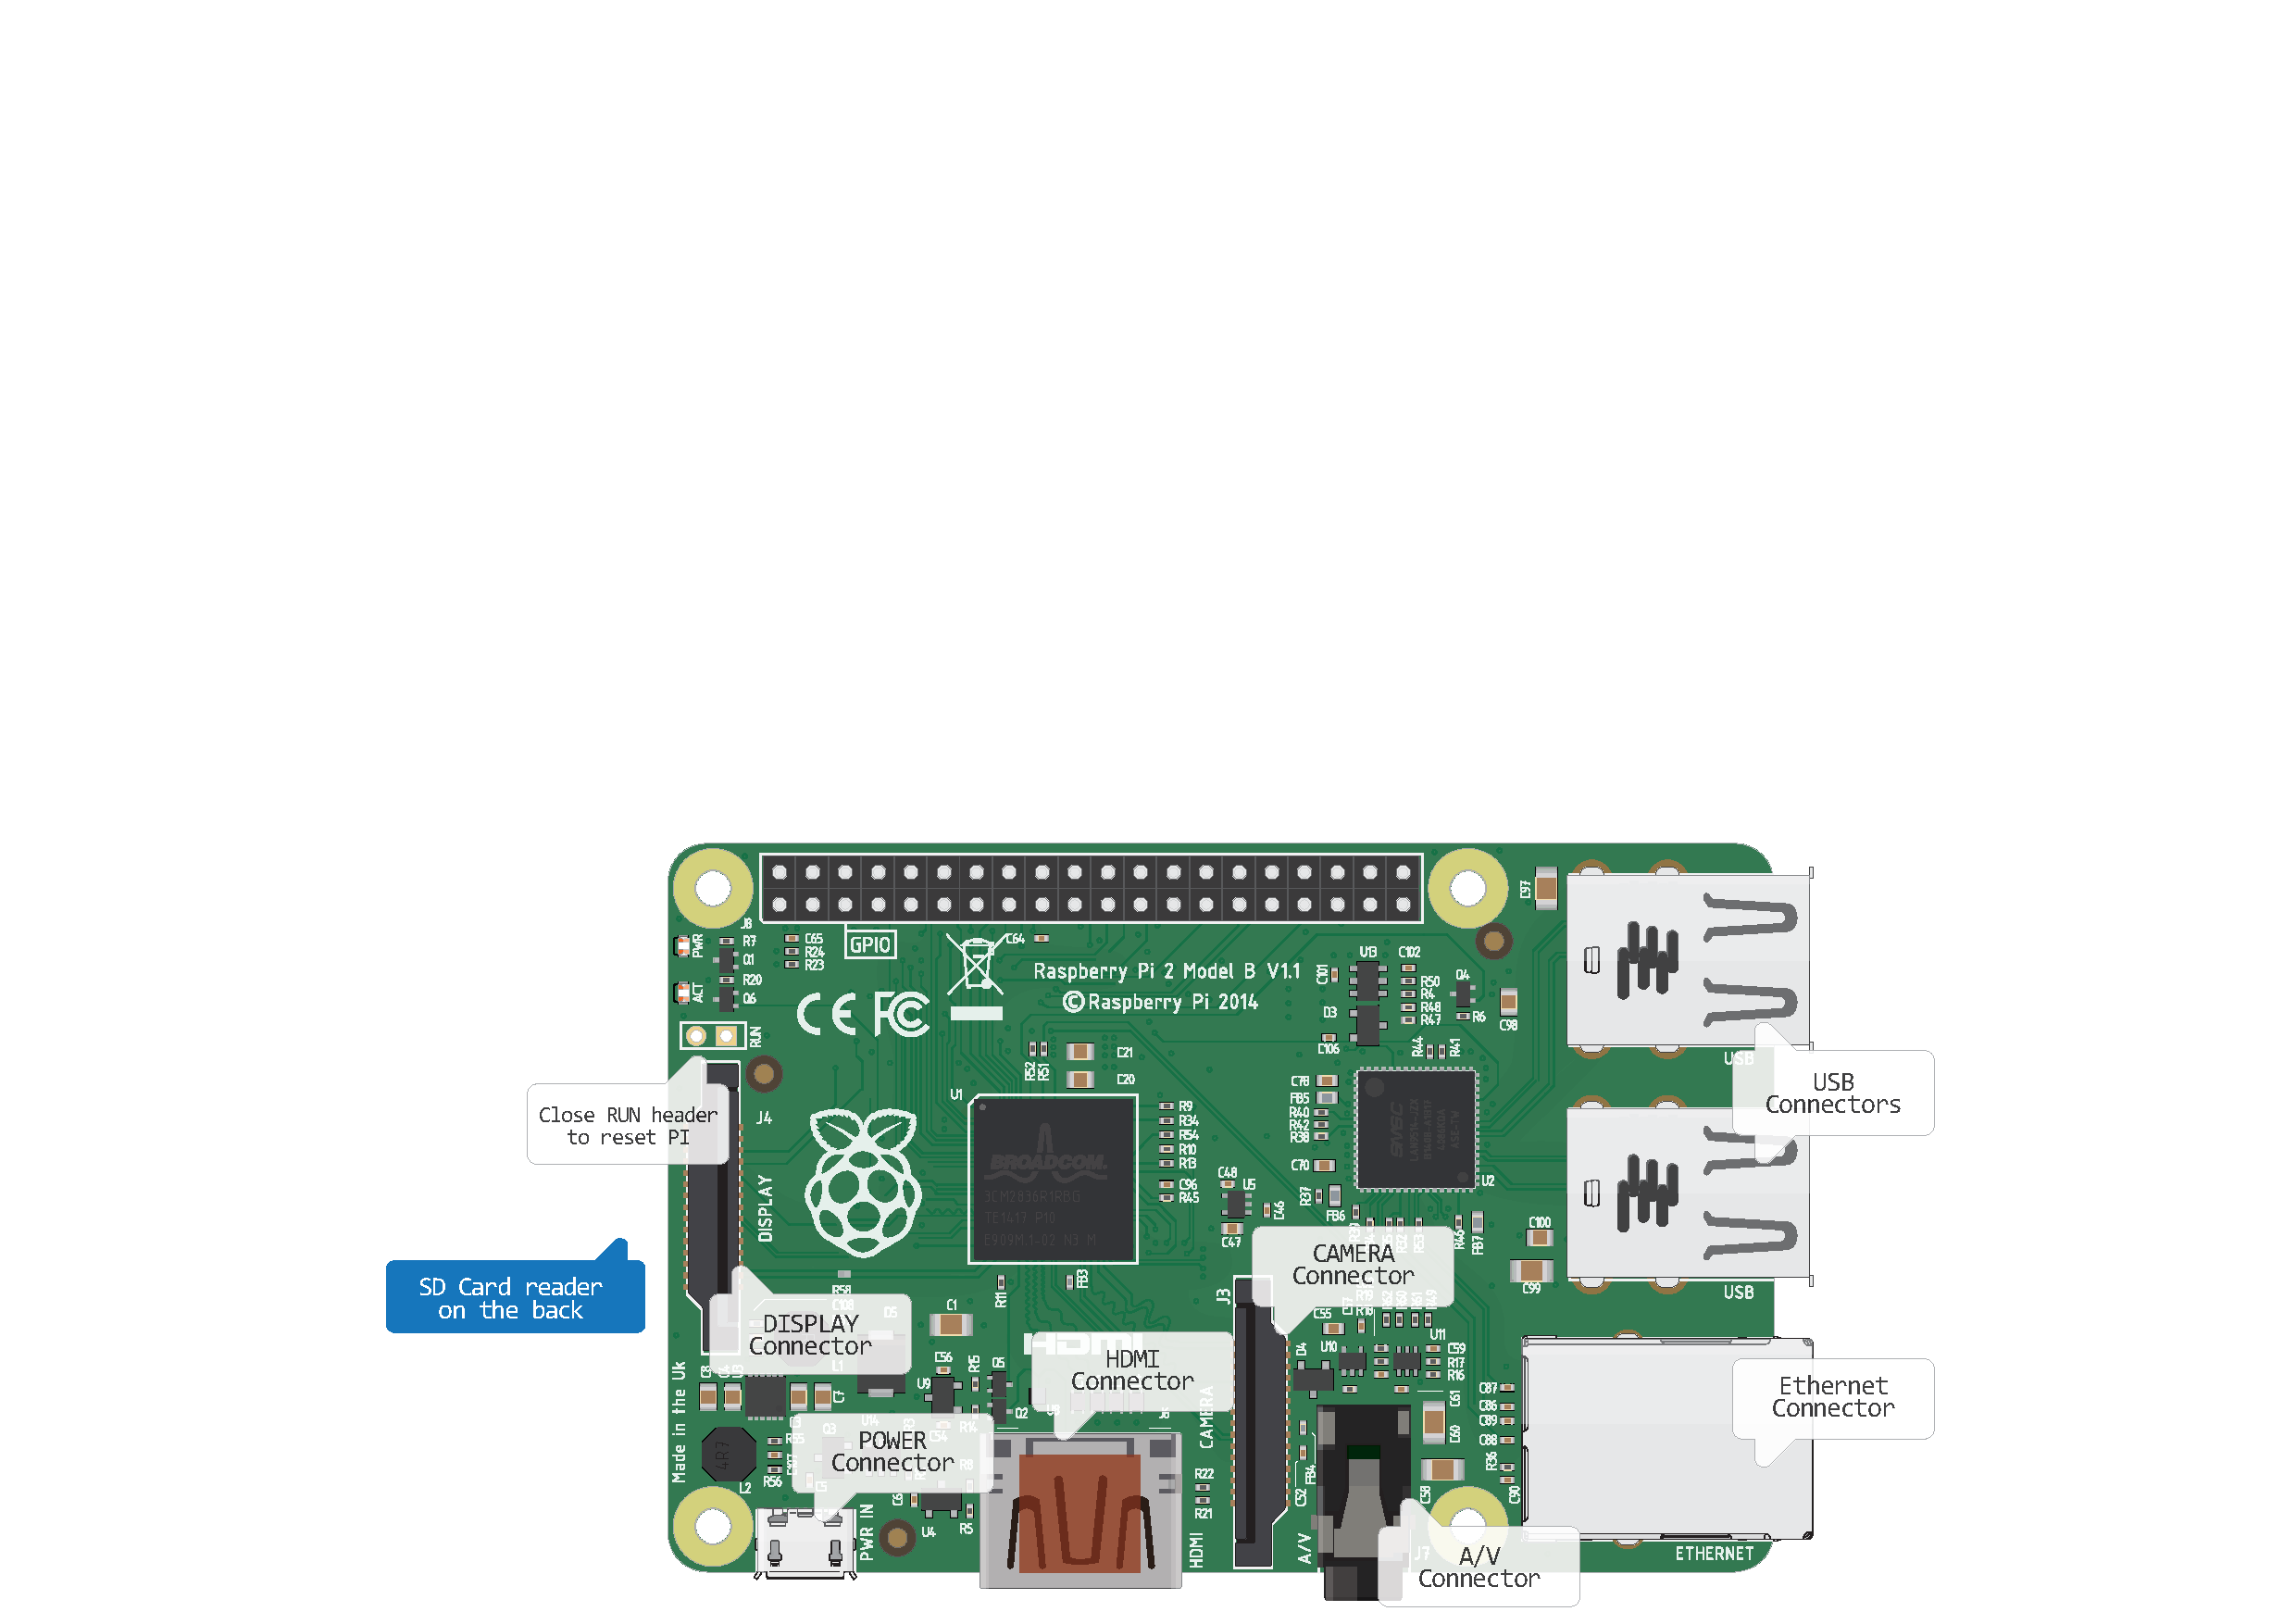
\includegraphics[width=6in]{figures/rasp.pdf}
\caption{Raspberry Pi二代B型}
\label{RASP_EPS}
\end{figure}
系统选择上,本文选择使用树莓派基金会的Debian系统,Linux内核版本为3.18\footnote{内核源码下载地址:\url{https://github.com/raspberrypi/linux}}。内核调试方案则选择使用KGDB调试工具,支持内核源码级别调试。
\subsection{Netfilter}
NC层实施方案有两种。第一种是直接在内核的TCP协议源码上更改,添加我们的NC层各个模块,然后再编译内核源码;第二种则是利用Linux内核提供给用户用于处理网络封包的框架——Netfilter,很多防火墙软件都是基于Netfilter开发的。考虑到工程复杂度,本文选择的是Netfilter框架。
\begin{figure}[htbp]
	\centering
	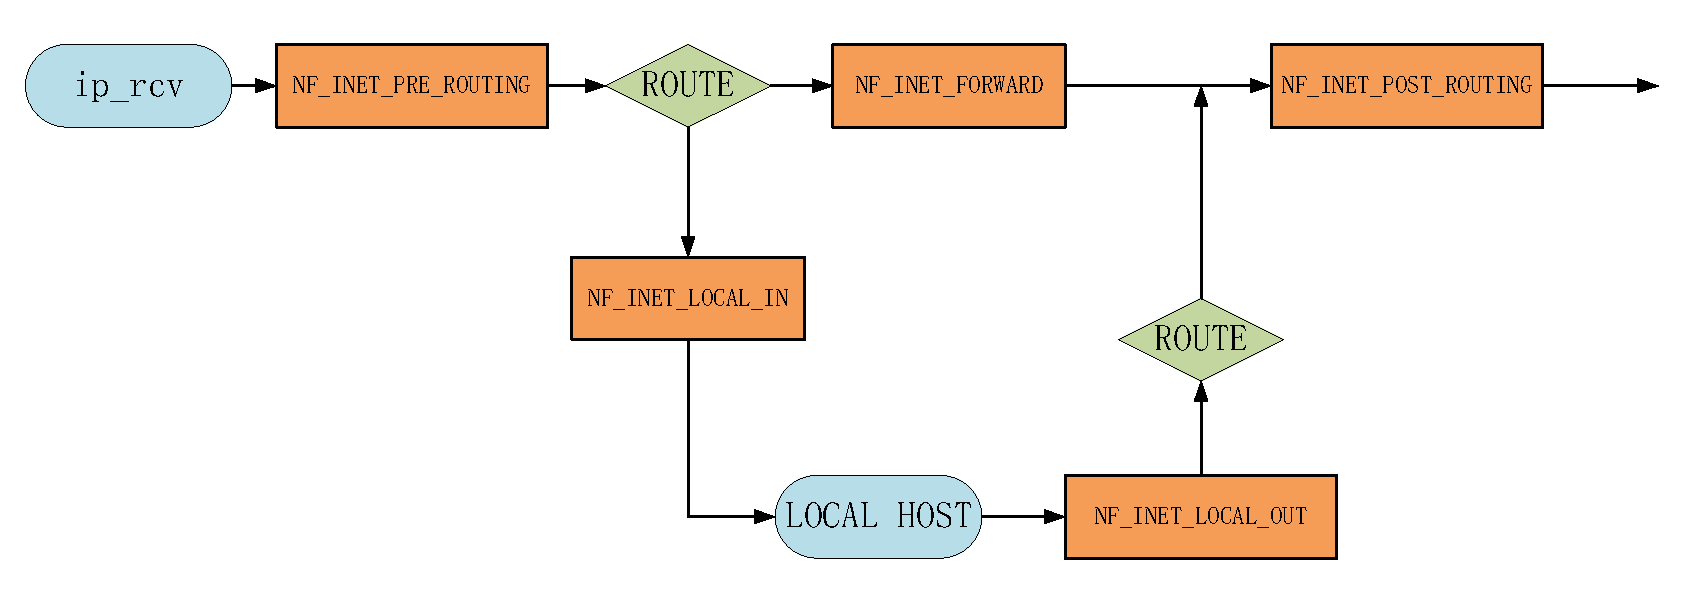
\includegraphics[width=6in]{figures/Netfilter.eps}
	\caption{Netfilter框架结构}
	\label{NETFILTER_EPS}
\end{figure}
Linux中最常用、最基本的防火墙软件称为$iptables$。$iptables$防火墙通过与Linux内核网络协议栈的包过滤钩子交互来工作。这些内核钩子被称为Netfilter框架。Linux系统中允许注册钩子程序的点有5个。数据包在路过Linux的网络协议栈时( 出去或者进来 ) 将触发这些钩子,允许注册这些钩子的函数处理处在钩子点处的报文。数据包所触发的钩子取决于数据包是传入还是传出,数据包的目的地,以及数据包在上一个钩子点是否被丢弃或拒绝。
\par
以下钩子表示网络协议栈中有标准定义的钩子点:
\begin{itemize}[leftmargin=.5in]
	\item \textbf{NF\_IP\_PRE\_ROUTING}:数据包在进入协议栈之后,在对这个数据包作出路由决定之前,会触发这个钩子。
	\item \textbf{NF\_IP\_LOCAL\_IN}:如果一个数据包是送往本机的,那么在作出这个路由决定之后,就会触发这个钩子。
	\item \textbf{NF\_IP\_FORWARD}:如果一个数据包经过路由判定是送往其他机器的,那么就会触发这个钩子。
	\item \textbf{NF\_IP\_POST\_ROUTING}:在数据包离开本机之前,会触发这个钩子。触发这个钩子的数据包包括从本机发往网络的包和仅仅是经过本机的路由判定后发往网络中其他机器的报文。
\end{itemize}
\par
图\ref{NETFILTER_EPS}展示的是Netfilter的框架。想要在这些钩子点注册的内核模块还需要提供一个优先级,用于决定在触发这个钩子时,按照一个什么顺序执行挂载在这些钩子上的模块。
\section{系统框架}
图\ref{JIAGOU_EPS}展示的是TCP/NC的实现架构,虚线框内的就是NC层。对于从TCP层下来的报文,首先要根据TCP报文头部信息判定是何种报文。如果是控制报文,如TCP连接建立的三次握手、RST报文,则交由控制报文处理模块进行分类处理。这些控制报文没有包含数据,无需经过编解码即可发往IP层。如果从TCP层下来的是数据报文,则需要被送到编码模块进行编码。编码后的数据包需要添加NC头部,填写NC层的控制信息,如编码包的系数、长度等。NC报文组包完毕后被发往IP层。对于从TCP层下来的纯ACK报文( 不带数据 ),也需要添加NC头部,主要是为了不浪费向对端传递NC层的相关信息的机会。
\par
从IP层上来的报文也需要经过数据包类别判定。控制报文直接交给控制报文处理模块处理,然后交给上层TCP层。对于纯ACK则在提取NC层有用信息后再交付给上层TCP层。数据报文则送到解码模块进行解码,不论解码成功,亦或是仅仅看到某个报文( see a packet ),解码模块都需要和NC层控制单元交互信息。
\begin{figure}[htbp]
	\centering
	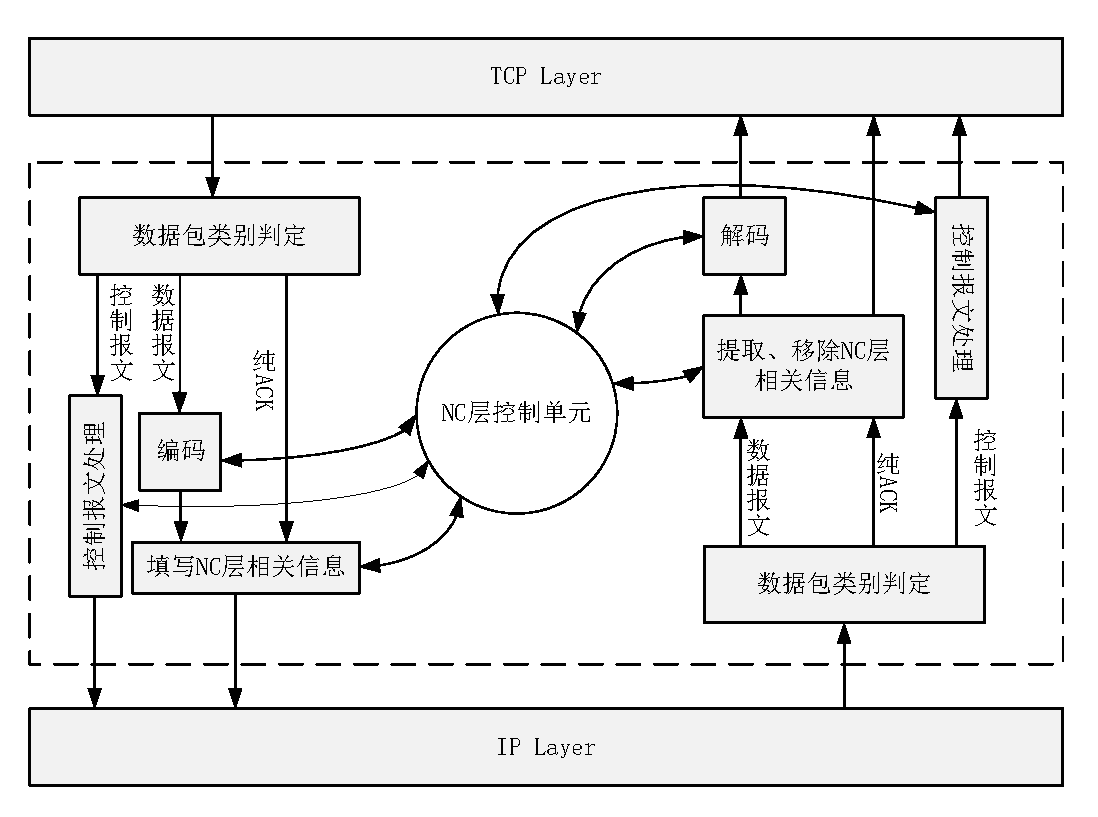
\includegraphics[width=6in]{figures/jiagou.eps}
	\caption{TCP/NC实现架构}
	\label{JIAGOU_EPS}
\end{figure}

